\documentclass[11pt,a4paper]{article}
\usepackage[utf8]{inputenc}
\usepackage[T1]{fontenc}
\usepackage{tgpagella}
\usepackage[spanish]{babel}
\usepackage{geometry}
\usepackage{booktabs}
\usepackage{xcolor}
\usepackage{titlesec}
\usepackage{fancyhdr}
\usepackage[parfill]{parskip}
\usepackage[expansion=false]{microtype}
\usepackage{hyperref}
\usepackage{setspace}
\usepackage{graphicx}
\usepackage{needspace}
\widowpenalty=10000
\clubpenalty=10000
\displaywidowpenalty=10000

\geometry{top=3.0cm,bottom=3.0cm,left=3.5cm,right=3.5cm}
\setlength{\parskip}{0.65em}
\setlength{\parindent}{0em}

\definecolor{azulai}{RGB}{30,80,140}
\definecolor{doradoai}{RGB}{140,90,0}
\definecolor{grisai}{RGB}{70,70,70}

\titleformat{\section}{\Large\bfseries\color{azulai}}{}{0em}{}[{\color{azulai}\titlerule[0.5pt]}]
\titlespacing*{\section}{0pt}{1.4em}{0.5em}

\titleformat{\subsection}{\large\bfseries\color{doradoai}}{}{0em}{}
\titlespacing*{\subsection}{0pt}{1.0em}{0.35em}

\titleformat{\subsubsection}{\normalsize\bfseries\color{grisai}}{}{0em}{}
\titlespacing*{\subsubsection}{0pt}{0.7em}{0.25em}

\pagestyle{fancy}\fancyhf{}
\rhead{\textcolor{grisai}{\small Raquel Pain — Arquitectura Interna}}
\lhead{\textcolor{grisai}{\small Urano · Neptuno · Plutón}}
\cfoot{\textcolor{grisai}{\small\thepage}}
\renewcommand{\headrulewidth}{0.3pt}

\hypersetup{colorlinks=true,linkcolor=azulai,urlcolor=azulai}
\setstretch{1.25}
\tolerance=1500
\emergencystretch=4em

\begin{document}

% ── Portada ──────────────────────────────────────────────────────────────────
\begin{titlepage}
  \centering
  \vspace*{1.5cm}
  {\Huge\bfseries\color{azulai} Urano · Neptuno · Plutón}\\[0.5cm]
  {\large\color{grisai} Arquitectura Interna}\\[0.3cm]
  {\small\itshape\color{grisai} Procesos profundos de cambio, sensibilidad y transformación}\\[2cm]
  {\huge\color{doradoai} Raquel Pain}\\[1.5cm]
  {\Large 07/05/1985 \quad 18:20}\\[0.3cm]
  {\Large Pamplona, España}\\[0.3cm]
  {\normalsize Lat: 42.8157° \quad Lon: -1.6522° \quad UTC+02:00}\\[0.3cm]
  {\normalsize Ascendente: Libra 14°36' \quad
    MC: Cáncer 17°21'}\\[2cm]
  \begin{tabular}{ll}
    \textbf{Urano:}   & Sagitario — Casa 3 17°09' (retrógrado)  \\
    \textbf{Neptuno:} & Capricornio — Casa 3 3°20' (retrógrado) \\
    \textbf{Plutón:}  & Escorpio — Casa 1 2°58' (retrógrado) \\
  \end{tabular}\\[2cm]
  \vfill
  {\small Generado el 20/05/2026}
\end{titlepage}

\tableofcontents
\newpage

% ── Datos de referencia ───────────────────────────────────────────────────────
\section{Datos de referencia}

\begin{center}
\begin{tabular}{llll}
  \toprule
  \textbf{Planeta} & \textbf{Signo} & \textbf{Casa} & \textbf{Posición} \\
  \midrule
  Urano (retrógrado)    & Sagitario   & 3   & 17°09'  \\
  Neptuno (retrógrado) & Capricornio  & 3  & 3°20' \\
  Plutón (retrógrado)  & Escorpio  & 1  & 2°58' \\
  Sol              & Tauro  & 8  & 17°02' \\
  Luna             & Sagitario & 3 & 26°31' \\
  Ascendente       & Libra          & ---                   & 14°36' \\
  Medio Cielo      & Cáncer           & ---                   & 17°21' \\
  \bottomrule
\end{tabular}
\end{center}

\vspace{0.5cm}
\textbf{Aspectos relevantes:}

\begin{center}
\begin{tabular}{lllll}
  \toprule
  \textbf{Planeta 1} & \textbf{Asp.} & \textbf{Planeta 2} & \textbf{Tipo} & \textbf{Orbe} \\
  \midrule
  Neptuno & sex & Plutón & Sextil & 0.4° \\
  Urano & sex & Júpiter & Sextil & 1.4° \\
  Urano & tri & Mercurio & Trígono & 4.0° \\
  Neptuno & cua & Venus & Cuadratura & 5.5° \\
  Lilith & opo & Plutón & Oposición & 5.8° \\
  Lilith & tri & Neptuno & Trígono & 6.1° \\
  Neptuno & conj & Luna & Conjunción & 6.8° \\
  Urano & conj & Luna & Conjunción & 9.4° \\
  \bottomrule
\end{tabular}
\end{center}

\begin{center}
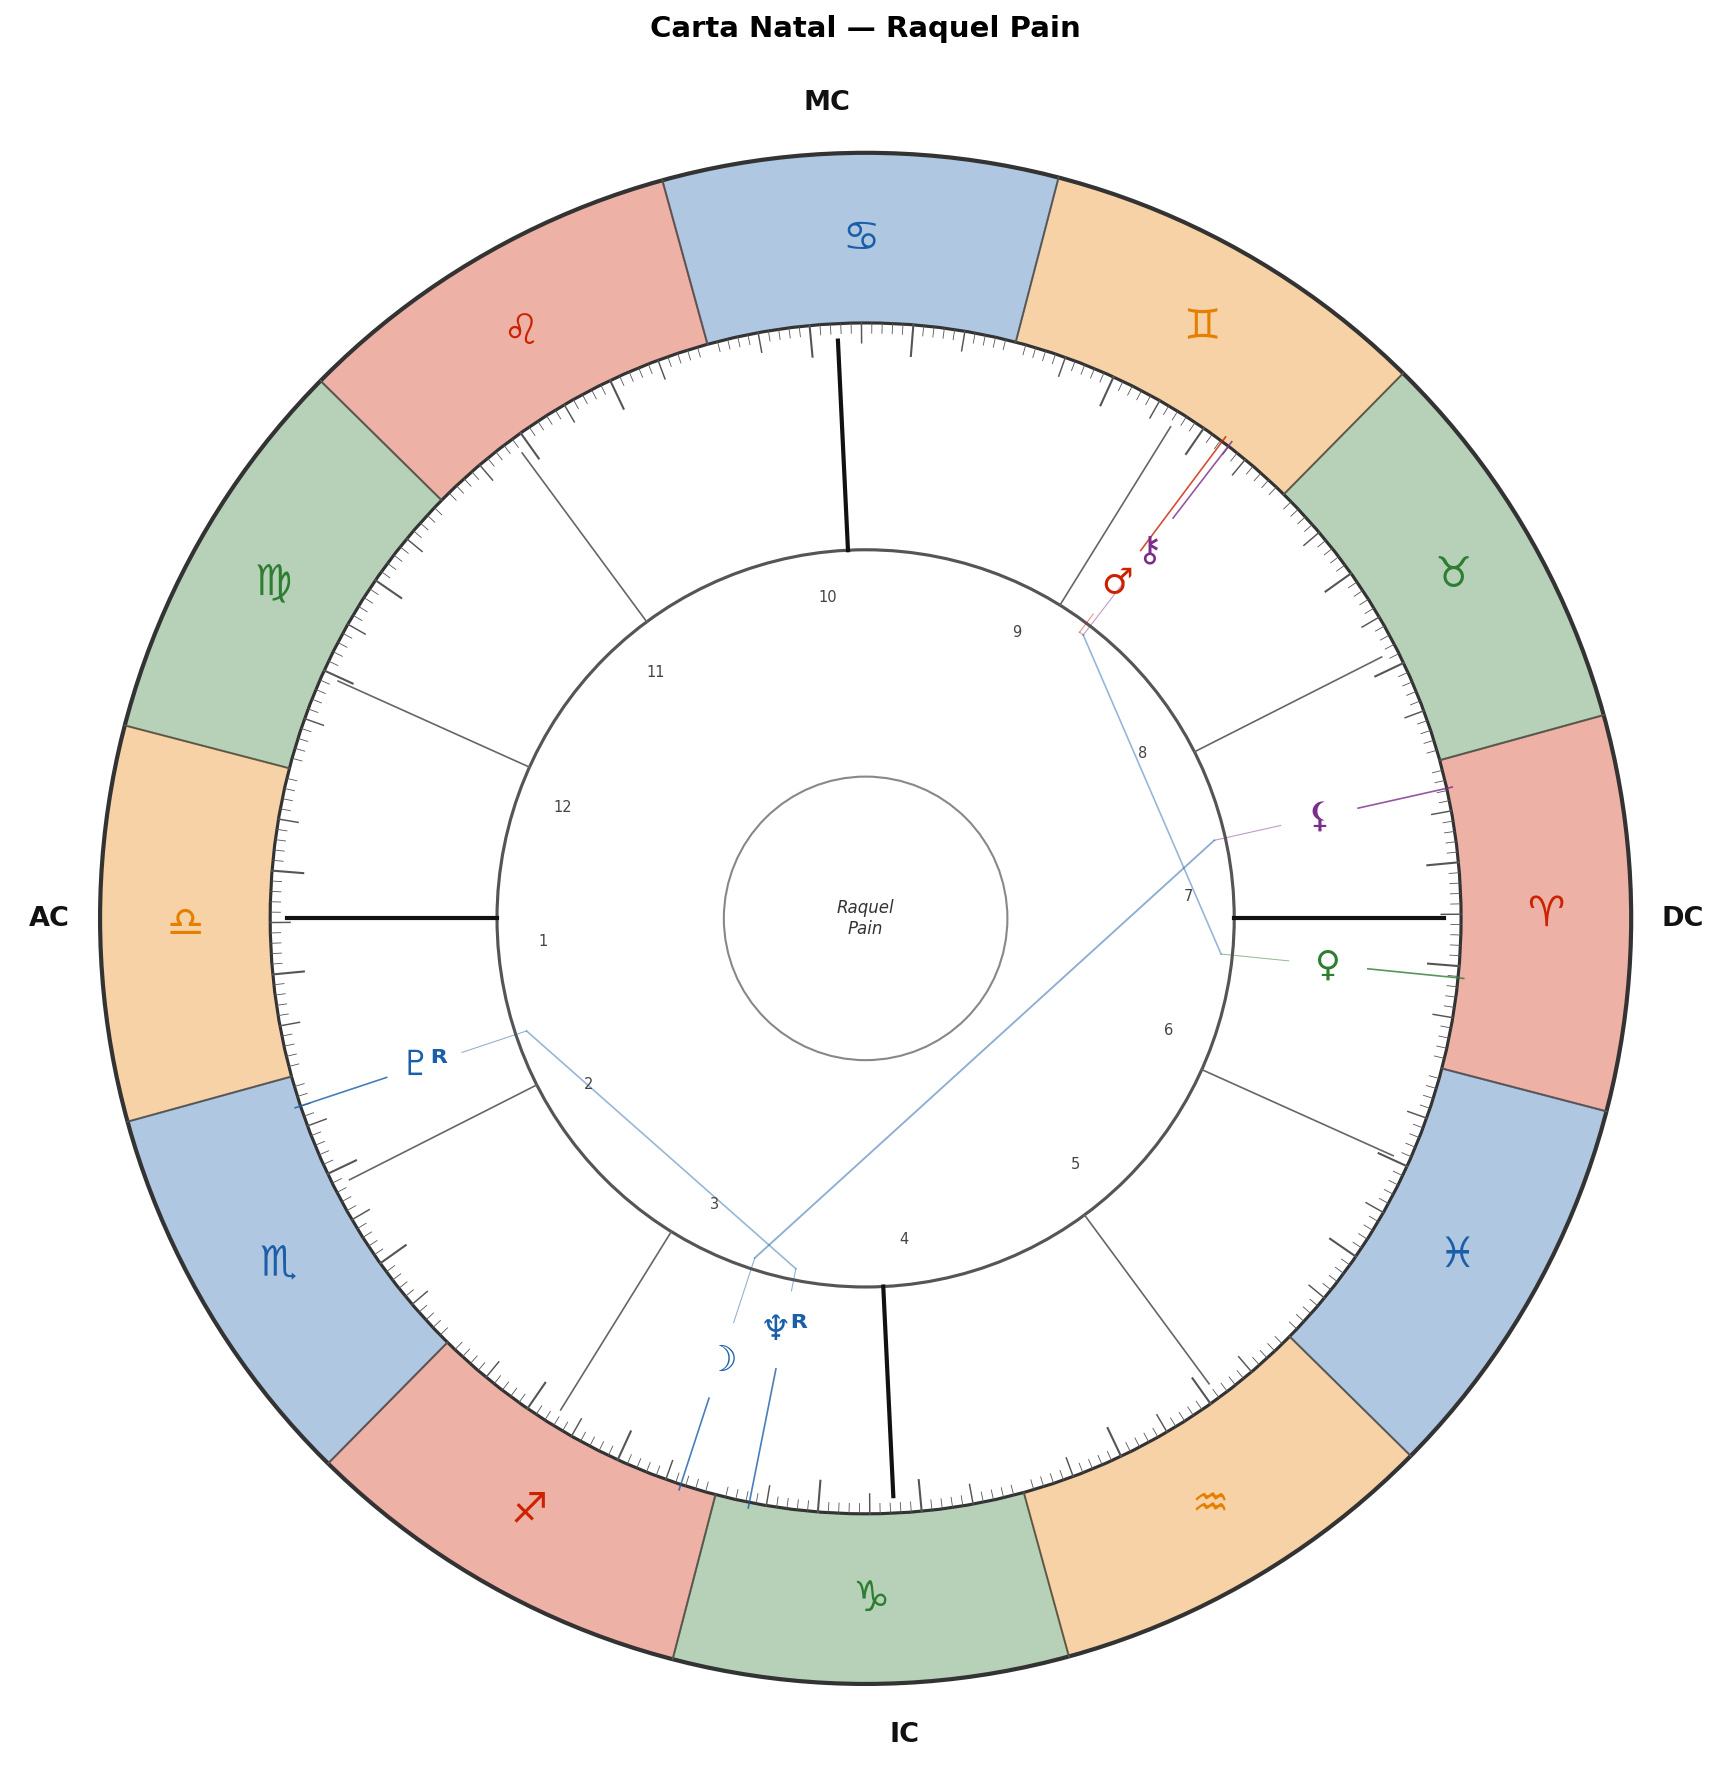
\includegraphics[width=0.72\textwidth]{Raquel_Pain_rueda.png}
\end{center}

\Needspace{3\baselineskip}


% ── Interpretación ────────────────────────────────────────────────────────────
\section{Interpretación — Arquitectura Interna}

\begin{center}
{\small\itshape
No se trata de describir la personalidad. Se trata de mostrar qué procesos\\
de cambio, sensibilidad y transformación pueden activarse en tu vida.
}
\end{center}

\vspace{0.8cm}
\Needspace{5\baselineskip}

% ── 1. Marco general ──────────────────────────────────────────────────────────
\subsection{1. Marco general}

Urano, Neptuno y Plutón no describen lo más cotidiano o visible de tu carta. Muestran procesos más profundos, menos controlables, que pueden modificar tu forma de vivir, sostenerte y atravesar determinadas etapas.

Urano en Sagitario, Casa 3: muestra dónde aparecen cambios, interrupciones o necesidad de libertad. Cuando se activa, algo que antes funcionaba puede dejar de hacerlo igual.
Neptuno en Capricornio, Casa 3: muestra dónde los límites se vuelven más sensibles, difusos o permeables. Cuando se activa, algo que parecía claro puede perder forma.
Plutón en Escorpio, Casa 1: muestra dónde aparecen procesos intensos de transformación. Cuando se activa, algo que se sostenía de una manera ya no puede seguir igual.

Aspectos activos con planetas personales: Urano–Luna en conjunción (orbe 9.37°), Urano–Mercurio en trígono (orbe 4.04°), Neptuno–Luna en conjunción (orbe 6.82°), Neptuno–Venus en cuadratura (orbe 5.53°).

\vspace{0.8cm}
\Needspace{5\baselineskip}


% ── 2. Urano ──────────────────────────────────────────────────────────────────
\subsection{2. Urano — Ruptura y cambio de patrón}

\subsubsection*{Urano en Sagitario — Casa 3 (retrógrado)}

Urano en Sagitario muestra necesidad de revisar creencias, direcciones y formas de entender la vida. Los cambios suelen aparecer cuando una visión deja de darte sentido o amplitud.

Puede haber giros fuertes en ideas, estudios, filosofía de vida o proyectos que parecían definir tu dirección. A veces cambias de horizonte muy rápido porque necesitas volver a sentir apertura y movimiento.

El aprendizaje pasa por permitir nuevas perspectivas sin perder completamente la continuidad de tu camino.

Urano en Casa 3 muestra una mente rápida, inquieta y difícil de mantener dentro de formas demasiado repetitivas. Necesitas revisar constantemente la manera en que piensas, aprendes o te comunicas.

Puede haber cambios bruscos de ideas, intereses o maneras de entender las cosas. A veces haces conexiones muy rápidas, pero también puedes perder interés igual de rápido.

El aprendizaje está en permitir movimiento mental sin desconectarte completamente de lo que quieres desarrollar.

Urano está retrógrado. Los cambios tienden a sentirse primero por dentro. Puede pasar tiempo antes de que se vean fuera, pero internamente algo ya está moviéndose, reorganizándose o dejando de funcionar como antes.

Urano en conjunción con la Luna hace que los cambios afecten directamente a tu mundo emocional y a la forma en que buscas estabilidad interna. Puede costarte sostener durante mucho tiempo estados emocionales demasiado previsibles o estructuras afectivas rígidas.

A veces hay cambios emocionales rápidos, necesidad de más espacio o sensación de que algo interno se mueve antes de que puedas entenderlo del todo.

El aprendizaje está en desarrollar estabilidad emocional sin intentar eliminar completamente el cambio.

Urano en trígono a Mercurio facilita pensar de forma original, flexible y creativa. Las nuevas ideas suelen aparecer con bastante naturalidad.

Existe capacidad para adaptarte rápido a cambios, aprender cosas nuevas y encontrar soluciones poco convencionales.

El aprendizaje está en dar continuidad a las ideas para que puedan desarrollarse realmente.

\vspace{0.8cm}
\Needspace{5\baselineskip}

% ── 3. Neptuno ────────────────────────────────────────────────────────────────
\subsection{3. Neptuno — Disolución y pérdida de forma}

\subsubsection*{Neptuno en Capricornio — Casa 3 (retrógrado)}

Neptuno en Capricornio vuelve más difusos los límites relacionados con estructura, responsabilidad y dirección de vida. Puede costarte distinguir qué construcciones siguen teniendo sentido y cuáles mantienes solo por inercia.

A veces sostienes demasiado tiempo responsabilidades, trabajos o formas de vida que internamente ya se han vaciado. También puede haber sensación de desorientación respecto al futuro o al lugar que ocupas.

El aprendizaje pasa por construir una estructura más coherente con lo que realmente tiene vida para ti.

Neptuno en Casa 3 puede hacer que la mente funcione de forma muy intuitiva y asociativa, pero también bastante dispersa en algunos momentos.

Puede haber dificultad para organizar ideas, explicar con precisión lo que quieres decir o mantener claridad mental cuando hay demasiada información o estímulos.

El aprendizaje pasa por desarrollar más foco y claridad sin perder sensibilidad ni imaginación.

Neptuno está retrógrado. La sensibilidad, la confusión o la pérdida de claridad tienden a vivirse primero internamente. Puede costarte detectar desde fuera cuándo algo está perdiendo forma, porque el proceso empieza en capas más silenciosas.

Neptuno en conjunción con la Luna intensifica muchísimo la sensibilidad emocional. Puede costarte distinguir claramente qué sientes tú y qué estás absorbiendo del entorno.

A veces hay mucha empatía, intuición y conexión emocional, pero también etapas de confusión, desbordamiento o sensación de perderte en lo que sienten otras personas.

El aprendizaje está en desarrollar límites emocionales más conscientes sin cerrar la sensibilidad.

Neptuno en cuadratura a Venus genera tensión entre necesidad de vínculo y dificultad para mantener claridad emocional y afectiva. Una parte de ti busca conexión ideal y otra necesita reconocer la realidad de lo que está viviendo.

Puede haber idealización de relaciones, dificultad para poner límites o tendencia a sostener vínculos poco claros durante demasiado tiempo.

El aprendizaje pasa por construir relaciones más conscientes sin cerrar la sensibilidad afectiva.

\vspace{0.8cm}
\Needspace{5\baselineskip}

% ── 4. Plutón ─────────────────────────────────────────────────────────────────
\subsection{4. Plutón — Intensidad y transformación profunda}

\subsubsection*{Plutón en Escorpio — Casa 1 (retrógrado)}

Plutón en Escorpio intensifica muchísimo los procesos emocionales profundos, la necesidad de transformación y el contacto con lo que no puede mantenerse en superficie. Las experiencias suelen vivirse con mucha intensidad.

Puede haber necesidad de controlar lo que ocurre internamente, miedo a perder poder o sensación de atravesar procesos que cambian completamente tu forma de vivir determinadas cosas.

El aprendizaje está en permitir transformación profunda sin vivir constantemente desde la tensión o el control.

Plutón en Casa 1 hace que los procesos de transformación afecten directamente a tu identidad, tu presencia y tu forma de posicionarte en la vida. Es difícil sostener durante mucho tiempo versiones de ti que ya no tienen verdad interna.

Puede haber etapas de cambios profundos en la manera de actuar, mostrarte o relacionarte con el entorno. También puedes generar impacto intenso en otras personas incluso sin buscarlo.

El aprendizaje está en permitir transformación sin vivir constantemente desde la tensión o la necesidad de control.

Plutón está retrógrado. La intensidad y la transformación tienden a dirigirse primero hacia dentro. Puede haber procesos profundos que no se ven claramente desde fuera hasta que ya han acumulado mucha fuerza.

\vspace{0.8cm}
\Needspace{5\baselineskip}

% ── 5. Integración ────────────────────────────────────────────────────────────
\subsection{5. Integración — Las tres fuerzas en tu carta}

Urano, Neptuno y Plutón actúan de formas distintas y no siempre coordinadas. Urano en Sagitario, Casa 3, muestra dónde aparecen cambios, interrupciones o necesidad de libertad. Cuando se activa, algo que antes funcionaba puede dejar de hacerlo igual. Neptuno en Capricornio, Casa 3, muestra dónde los límites se vuelven más sensibles, difusos o difíciles de sostener. Cuando se activa, algo que parecía claro puede perder forma. Plutón en Escorpio, Casa 1, muestra dónde aparecen procesos intensos de transformación. Cuando se activa, algo que sostenías de una manera ya no puede seguir igual.

Neptuno en Capricornio muestra una sensibilidad especial en ciertas áreas de tu vida: puedes mantener situaciones o estructuras mucho más tiempo del que realmente necesitas. Urano en Sagitario muestra cómo suelen producirse los cambios importantes: los cambios aparecen cuando cambia el impulso que te mueve. Plutón en Escorpio concentra la intensidad en procesos que no pueden quedarse igual indefinidamente: determinadas experiencias terminan empujándote a transformar algo en profundidad.

En determinados momentos, estas tres fuerzas pueden activarse de forma encadenada. Urano en Sagitario suele aparecer primero: los impulsos cambian antes de que puedas completar lo que habías iniciado. Después, Neptuno en Capricornio puede hacer que aparezca sensación de confusión, pérdida de claridad o dificultad para entender bien qué está pasando: lo que parecía sólido deja de sentirse tan claro o seguro. Finalmente, Plutón en Escorpio concentra la intensidad en aquello que ya no puede seguir igual: la intensidad se concentra en emociones profundas y vínculos importantes. Por eso, determinadas etapas pueden sentirse especialmente intensas: no estás viviendo una sola cosa, sino varios procesos moviéndose al mismo tiempo.

\vspace{0.8cm}
\Needspace{5\baselineskip}

% ── 6. Orientación ────────────────────────────────────────────────────────────
\subsection{6. Orientación}

\subsubsection*{Cuando Urano está activo}
Urano suele activarse cuando: aparecen impulsos repentinos de cambio o necesidad de romper con algo rápidamente. Esto suele sentirse especialmente en temas relacionados con la Casa 3.

\subsubsection*{Cuando Neptuno está activo}
Neptuno suele activarse cuando: lo que parecía seguro o estable deja de sentirse tan sólido. Esto suele sentirse especialmente en temas relacionados con la Casa 3.

\subsubsection*{Cuando Plutón está activo}
Plutón suele activarse cuando: emociones y vínculos importantes atraviesan procesos muy intensos de transformación. Esto suele sentirse especialmente en temas relacionados con la Casa 1.

\subsubsection*{Cuando no se reconocen}
Cuando estos procesos no se reconocen, es fácil vivirlos únicamente como problemas externos o mala suerte. Sin embargo, muchas veces están mostrando que algo necesita cambiar, redefinirse o transformarse más profundamente.

Intentar sostener exactamente igual algo que internamente ya está cambiando suele generar más desgaste, más confusión o más sensación de bloqueo.

\vspace{0.6cm}
Si estos procesos se ignoran durante mucho tiempo, suelen intensificarse. Urano puede traer cambios cada vez más bruscos. Neptuno puede aumentar la sensación de confusión, desgaste o pérdida de claridad. Plutón puede concentrar tanta intensidad que determinadas situaciones ya no puedan seguir sosteniéndose igual.

Por eso, reconocer antes lo que está cambiando suele ayudar a atravesar estas etapas con más consciencia y menos ruptura.

\vspace{1cm}
\begin{center}
{\small\itshape\color{grisai}
La astrología se usa aquí como lenguaje simbólico de observación, no como definición de la persona.\
Este documento es una aproximación funcional, no un diagnóstico.
}
\end{center}

\end{document}
